\setcounter{table}{0}          
\renewcommand{\thetable}{S\arabic{table}}

\setcounter{subsection}{0}
\renewcommand{\thesubsection}{S\arabic{subsection}}

\subsection{Supplementary Method: traditional sparsification approaches}\label{supp_met_1}
\subsubsection{Backbone extraction via disparity filter}\label{subsec:backbone}
The disparity filter~\cite{serrano2009extracting} identifies statistically significant edges by comparing observed edge weights to a null model of uniform weight distribution. For each disease node $i$ with degree $k_i$ (considering all edges), the probability that edge weight $w_{ij}$ could arise by chance under uniform redistribution is:
\begin{equation}\label{eq:disparity_filter}
\alpha_{ij} = (1 - p_{ij})^{k_i - 1}
\end{equation}
where $p_{ij} = w_{ij} / s_i$ is the proportion of node $i$'s total weight $s_i = \sum_j w_{ij}$ allocated to edge $(i,j)$.

Edges with $\alpha_{ij} < \alpha_{\text{sig}}$ (typically $\alpha_{\text{sig}} = 0.05$) are retained, indicating their weights are significantly larger than expected under uniform redistribution. This produces a sparse "backbone" network preserving the most statistically salient relationships.

We apply the disparity filter to $A^{\mathcal{D+R}}$ at significance level $\alpha_{\text{sig}} = 0.05/n_{pairs}$, where $n_{pairs} = 2760$. This approach resulted in an empty network, even when the significance level was increased to $\alpha_{\text{sig}} = 0.05$. 

\subsubsection{Locally adapted network sparsification}\label{subsec:lans}
The Locally Adapted Network Sparsification (LANS) method~\cite{marcaccioli2022locally} addresses limitations of global thresholding by adapting significance thresholds to local network topology. Building on the noise-corrected backbone extraction framework~\cite{foti2011nonparametric}, LANS estimates a node-specific null model that accounts for the local strength distribution of edges. For each node $i$, the method computes a local significance threshold based on the distribution of edge weights incident to that node. Specifically, for edge $(i,j)$ with weight $w_{ij}$, the local p-value is computed as:
\begin{equation}\label{eq:lans}
p_{ij}^{\text{local}} = P(W \geq w_{ij} | \mathcal{N}_i)
\end{equation}
where $\mathcal{N}_i$ denotes the neighborhood of node $i$ and the null distribution is estimated from the empirical distribution of weights in $\mathcal{N}_i$. Edges are retained if $p_{ij}^{\text{local}} < \alpha_{\text{sig}}$ for both nodes $i$ and $j$, ensuring that the edge is locally significant from both endpoints' perspectives. This adaptive approach is particularly effective for networks with heterogeneous degree distributions or highly variable edge weight patterns, as it avoids the assumption of a single global null model. Implementation was performed using the LANS R package~\cite{marcaccioli2022locally}. We applied LANS to the risk-adjusted similarity network $A^{(\mathcal{D}+\mathcal{R})}$ with significance level $\alpha_{\text{sig}} = 0.05/n_{pairs}$. However, this approach resulted in an extremely sparse network showed in Figure~\ref{SF:backboning} which retains only 10 edges (3.6\% retention rate), with several clinically central diseases, including diabetes mellitus, hypertension, and multiple valvular conditions, left isolated without any connections.

\setcounter{figure}{0}          
\renewcommand{\thefigure}{SM-F\arabic{figure}}

\begin{figure}[h!]
    \centering
    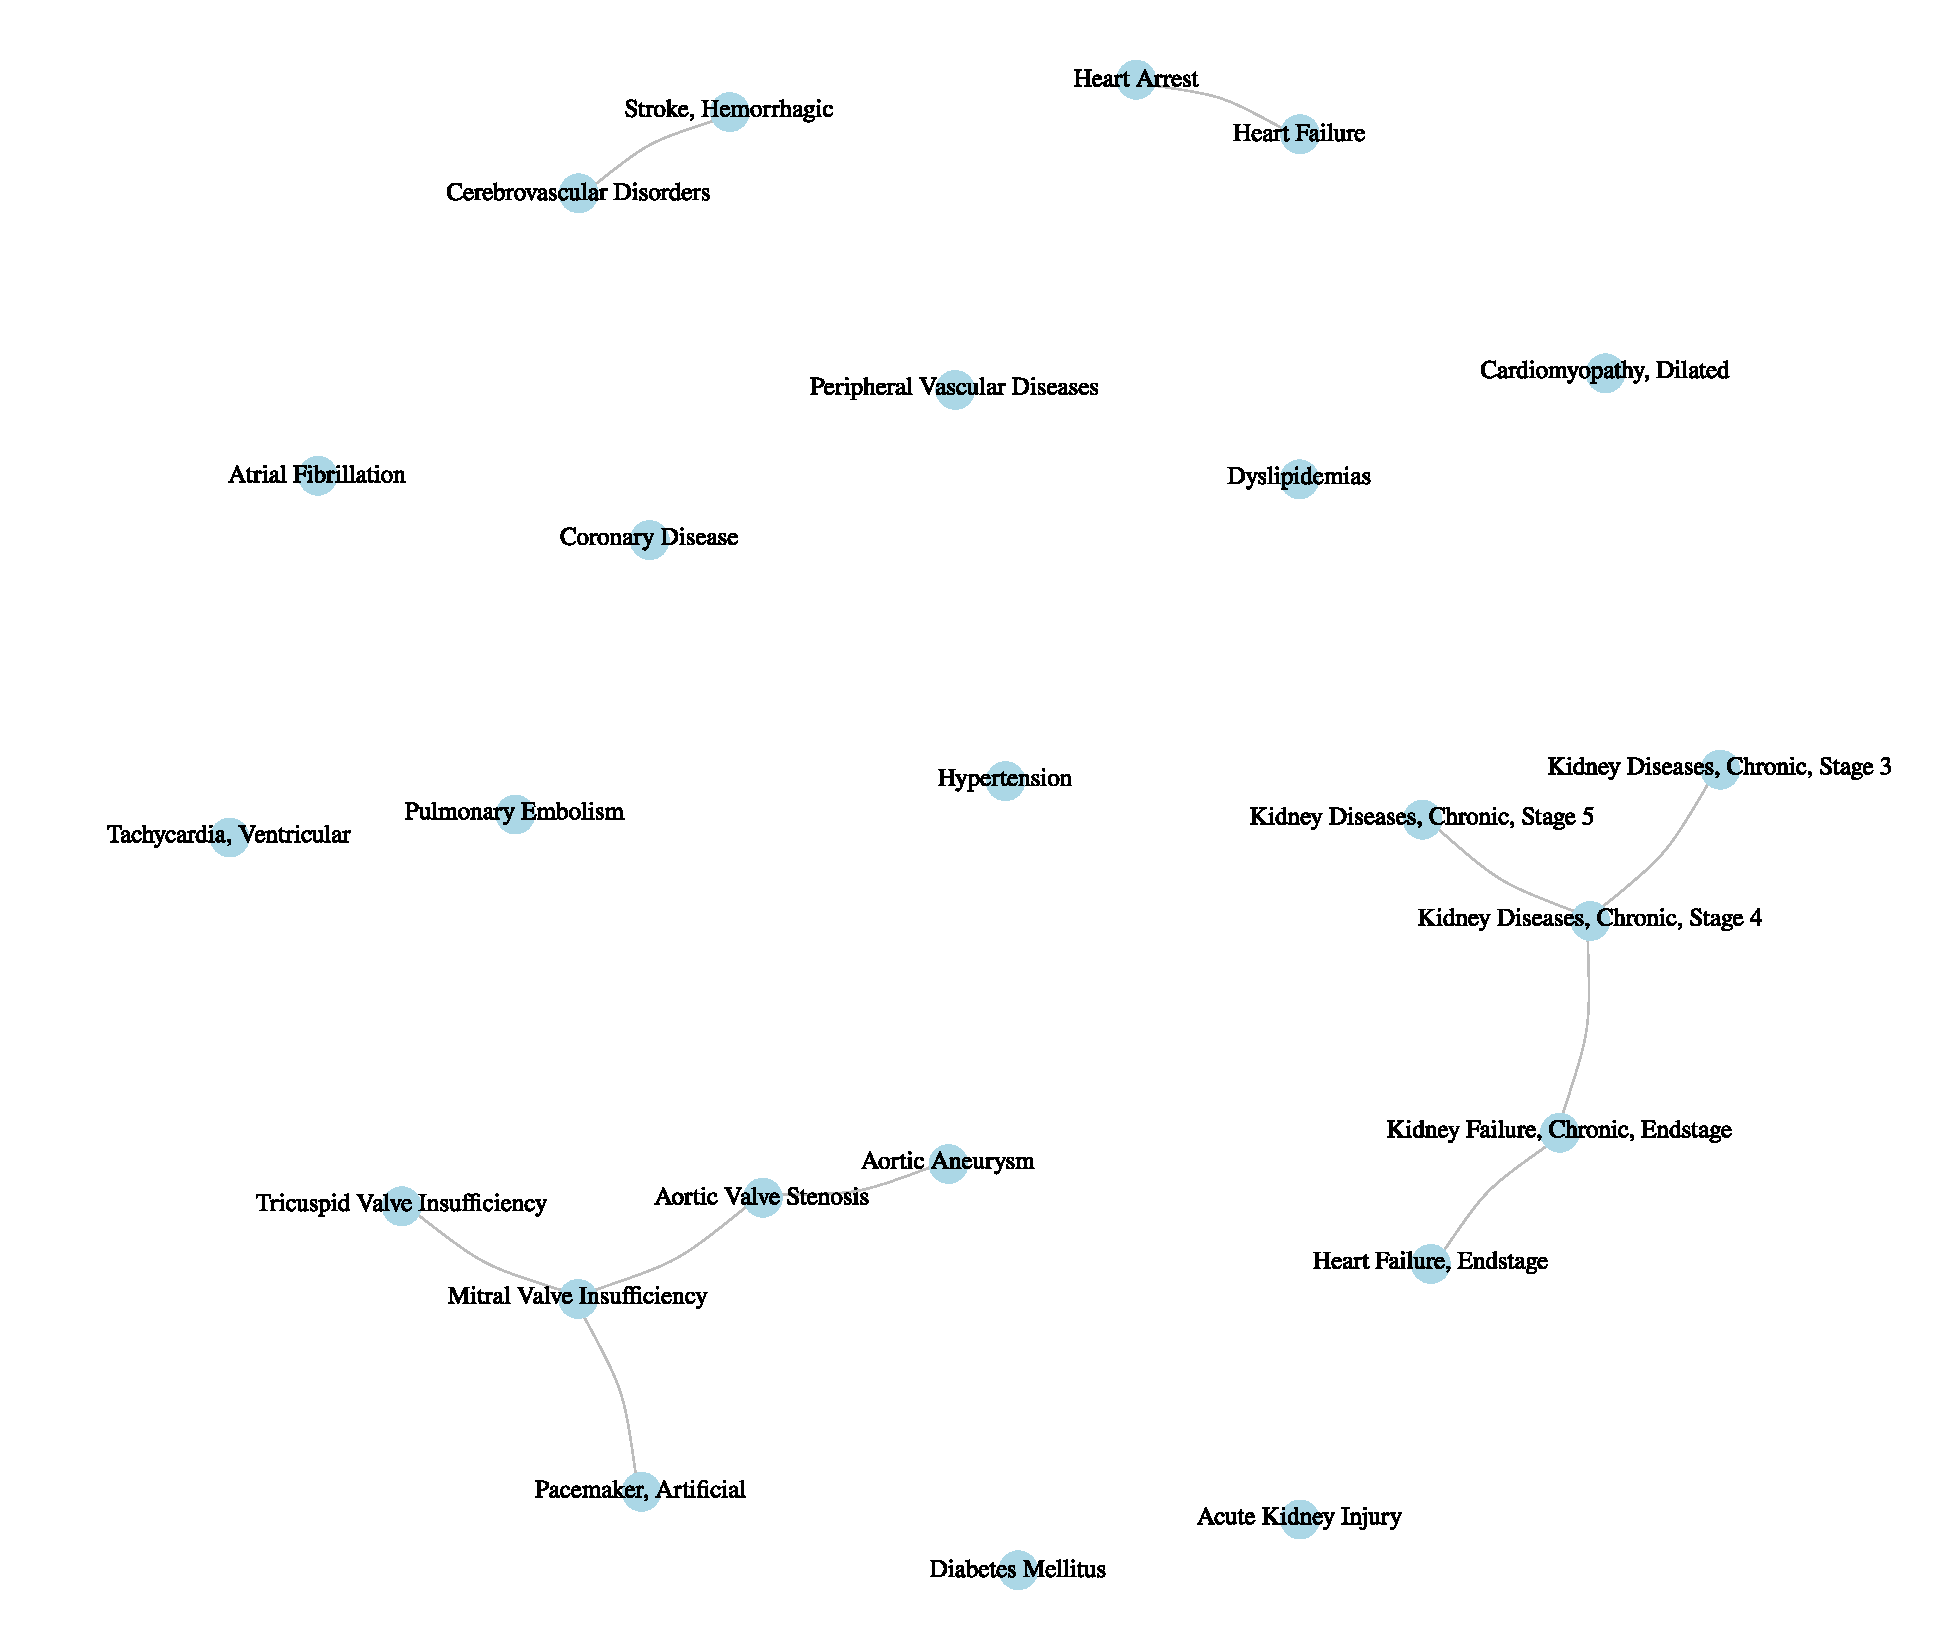
\includegraphics[width=1\textwidth]{Figures/Plots_backbone_main_par_comorb_diseases.pdf}
    \caption{Risk-adjusted Cardiometabolic disease network estimated via Locally adapted network sparsification.}
    \label{SF:backboning}
\end{figure}

This over-sparsification reflects a fundamental limitation of locally adaptive methods when applied to fully connected networks with relatively homogeneous, uniformly strong associations. In our similarity network, edge weights range narrowly (IQR range = 0.66-81, median = 0.74), with the majority of disease pairs exhibiting moderate-to-strong similarities. Under such conditions, local null models fail to distinguish genuine associations from background signal, as all edges appear locally significant or insignificant depending on arbitrary neighborhood definitions. The LANS method implicitly assumes substantial local heterogeneity in edge strengths, a condition not met in our embedding, based similarity network where diseases cluster into cohesive modules with consistently high internal similarities.

For these reasons, we concluded that statistically-based backboning methods are inadequate for sparsifying fully connected, homogeneously weighted similarity networks. This motivated our adoption of Gaussian Graphical Models (Section~\ref{subsec:sparsification}), which provide sparsification through conditional independence estimation rather than relying on assumptions about weight distribution heterogeneity.

\newpage
\subsection*{Supplementary Tables}
\begin{table}[h]
\centering
\caption{Cardiometabolic phenotypes definition with lifecourse incidence main diseases.}
\label{ST:table1}
\vspace{2mm}
\footnotesize Source: \url{https://htechnopole-my.sharepoint.com/:x:/r/personal/alessia_mapelli_fht_org/Documents/Dott/4th%20Year/SIS%202026/SIS_AM_NF_comorb_network/mapping_diseases.xlsx?d=we12a501ed7ec4cd49dea4ecebd599e85&csf=1&web=1&e=iBeF6F&nav=MTVfezY4RTgwMDg3LTNDRTUtNEM1OS1BM0RGLUJCNDgxRThFRDBDM30}
\end{table}

\begin{table}[h]
\centering
\caption{Risk factors phenotypes definition}
\label{ST:table2}
\vspace{2mm}
\footnotesize Source: \url{https://htechnopole-my.sharepoint.com/:x:/r/personal/alessia_mapelli_fht_org/Documents/Dott/4th%20Year/SIS%202026/SIS_AM_NF_comorb_network/mapping_diseases.xlsx?d=we12a501ed7ec4cd49dea4ecebd599e85&csf=1&web=1&e=XrGTiF&nav=MTVfezAwMDAwMDAwLTAwMDEtMDAwMC0wMDAwLTAwMDAwMDAwMDAwMH0}
\end{table}

\begin{table}[ht]
\centering
\caption{Shared risk factors for each disease pair across different sensitivity thresholds.}
\label{ST:shared_rf_sensitivity}
\small
\begin{tabular}{|l|c|c|c|c|c|c|}
\hline
\textbf{Disease Pair} & \textbf{0.5} & \textbf{0.6} & \textbf{0.7} & \textbf{0.72*} & \textbf{0.8} & \textbf{0.9} \\
\hline
TVI $\leftrightarrow$ DM   & 1.00 & 1.00 & 0.91 & \textbf{0.93} & 0.50 & 0.00 \\
AKI $\leftrightarrow$ HTN  & 1.00 & 0.99 & 0.91 & \textbf{0.82} & 0.50 & 0.00 \\
TVI $\leftrightarrow$ HTN  & 1.00 & 1.00 & 0.93 & \textbf{0.91} & 0.50 & 0.00 \\
VT $\leftrightarrow$ HTN   & 0.99 & 0.95 & 0.80 & \textbf{0.48} & 0.00 & 0.00 \\
AKI $\leftrightarrow$ DM   & 1.00 & 0.99 & 0.87 & \textbf{0.86} & 0.50 & 0.00 \\
MVI $\leftrightarrow$ DM   & 1.00 & 0.99 & 0.89 & \textbf{0.83} & 0.00 & 0.00 \\
MVI $\leftrightarrow$ HTN  & 1.00 & 0.95 & 0.78 & \textbf{0.64} & 0.00 & 0.00 \\
HTN $\leftrightarrow$ AVS  & 1.00 & 1.00 & 0.93 & \textbf{0.88} & 0.50 & 0.00 \\
TVI $\leftrightarrow$ CKD3 & 1.00 & 0.99 & 0.99 & \textbf{0.98} & 1.00 & 0.00 \\
MVI $\leftrightarrow$ CKD3 & 1.00 & 1.00 & 1.00 & \textbf{1.00} & 0.80 & 0.00 \\
MVI $\leftrightarrow$ CKD4 & 1.00 & 1.00 & 1.00 & \textbf{1.00} & 1.00 & 0.00 \\
MVI $\leftrightarrow$ CKD5 & 1.00 & 1.00 & 1.00 & \textbf{1.00} & 0.80 & 0.00 \\
CKD4 $\leftrightarrow$ TVI & 1.00 & 1.00 & 0.99 & \textbf{0.99} & 0.87 & 0.25 \\
PVD $\leftrightarrow$ TVI  & 1.00 & 0.97 & 0.97 & \textbf{0.97} & 0.96 & 0.00 \\
\hline
\textbf{Mean (SD)} & 0.99 (0.002) & 0.98 (0.02) & 0.93 (0.07) & \textbf{0.88 (0.15)} & 0.57 (0.36) & 0.02 (0.07) \\
\textbf{MW test p-value} & $8.51 \times 10^{-15}$ & $5.24 \times 10^{-15}$ & $6.43 \times 10^{-14}$ & $\mathbf{2.57 \times 10^{-14}}$ & $9.67 \times 10^{-11}$ & NA \\
\hline
\end{tabular}
\vspace{0.8em}
\footnotesize
\vspace{0.3em}
\footnotesize
\parbox{0.97\linewidth}{
\textit{Note:} Abbreviations: TVI = Tricuspid Valve Insufficiency, MVI = Mitral Valve Insufficiency, DM = Diabetes Mellitus, HTN = Hypertension, AKI = Acute Kidney Injury, VT = Ventricular Tachycardia, AVS = Aortic Valve Stenosis, CKD3-5 = Chronic Kidney Disease stages 3-5, PVD = Peripheral Vascular Diseases. *Main analysis threshold. MW test = Mann-Whitney U test\\
For $\tau = 0.9$ the Mann-Whitney U test was not applicable due to the high number of zeros.
}
\end{table}

\newpage

\begin{table}[h]
\centering
\begin{tabular}{lcc}
\hline
\textbf{Disease} & \textbf{Degree Centrality} & \textbf{Between Centrality} \\
\hline
Atrial Fibrillation & 1 & 1 \\
Acute Kidney Injury & 2 & 2 \\
Artificial Pacemaker & 3 & 3 \\
Coronary Disease & 4 & 4 \\
Aortic Valve Stenosis & 4 & 5 \\
Heart Failure & 6 & 6 \\
Dilated Cardiomyopathy & 11 & 7 \\
Chronic Kidney Failure Endstage & 7 & 8 \\
Tricuspid Valve Insufficiency & 11 & 9 \\
Diabetes Mellitus & 7 & 10 \\
Heart Failure, Endstage & 11 & 11 \\
Cerebrovascular Disorders & 11 & 12 \\
Stroke, Hemorrhagic & 9 & 13 \\
Chronic Kidney Diseases, Stage 4 & 17 & 14 \\
Chronic Kidney Diseases, Stage 5 & 17 & 15 \\
Peripheral Vascular Diseases & 15 & 16 \\
Heart Arrest & 9 & 17 \\
Hypertension & 15 & 18 \\
Tachycardia, Ventricular & 17 & 19 \\
Aortic Aneurysm & 20 & 20 \\
Mitral Valve Insufficiency & 21 & 21 \\
Pulmonary Embolism & 22 & 22 \\
Chronic Kidney Diseases, Stage 3 & 22 & 23 \\
Dyslipidemias & 22 & 24 \\
\hline
\end{tabular}
\caption{Centrality measures for diseases.}
\label{ST:centrality}
\end{table}

\setcounter{figure}{0}          
\renewcommand{\thefigure}{S\arabic{figure}}

\clearpage


\subsection*{Supplementary Figure}
\begin{figure}[H]
    \centering
    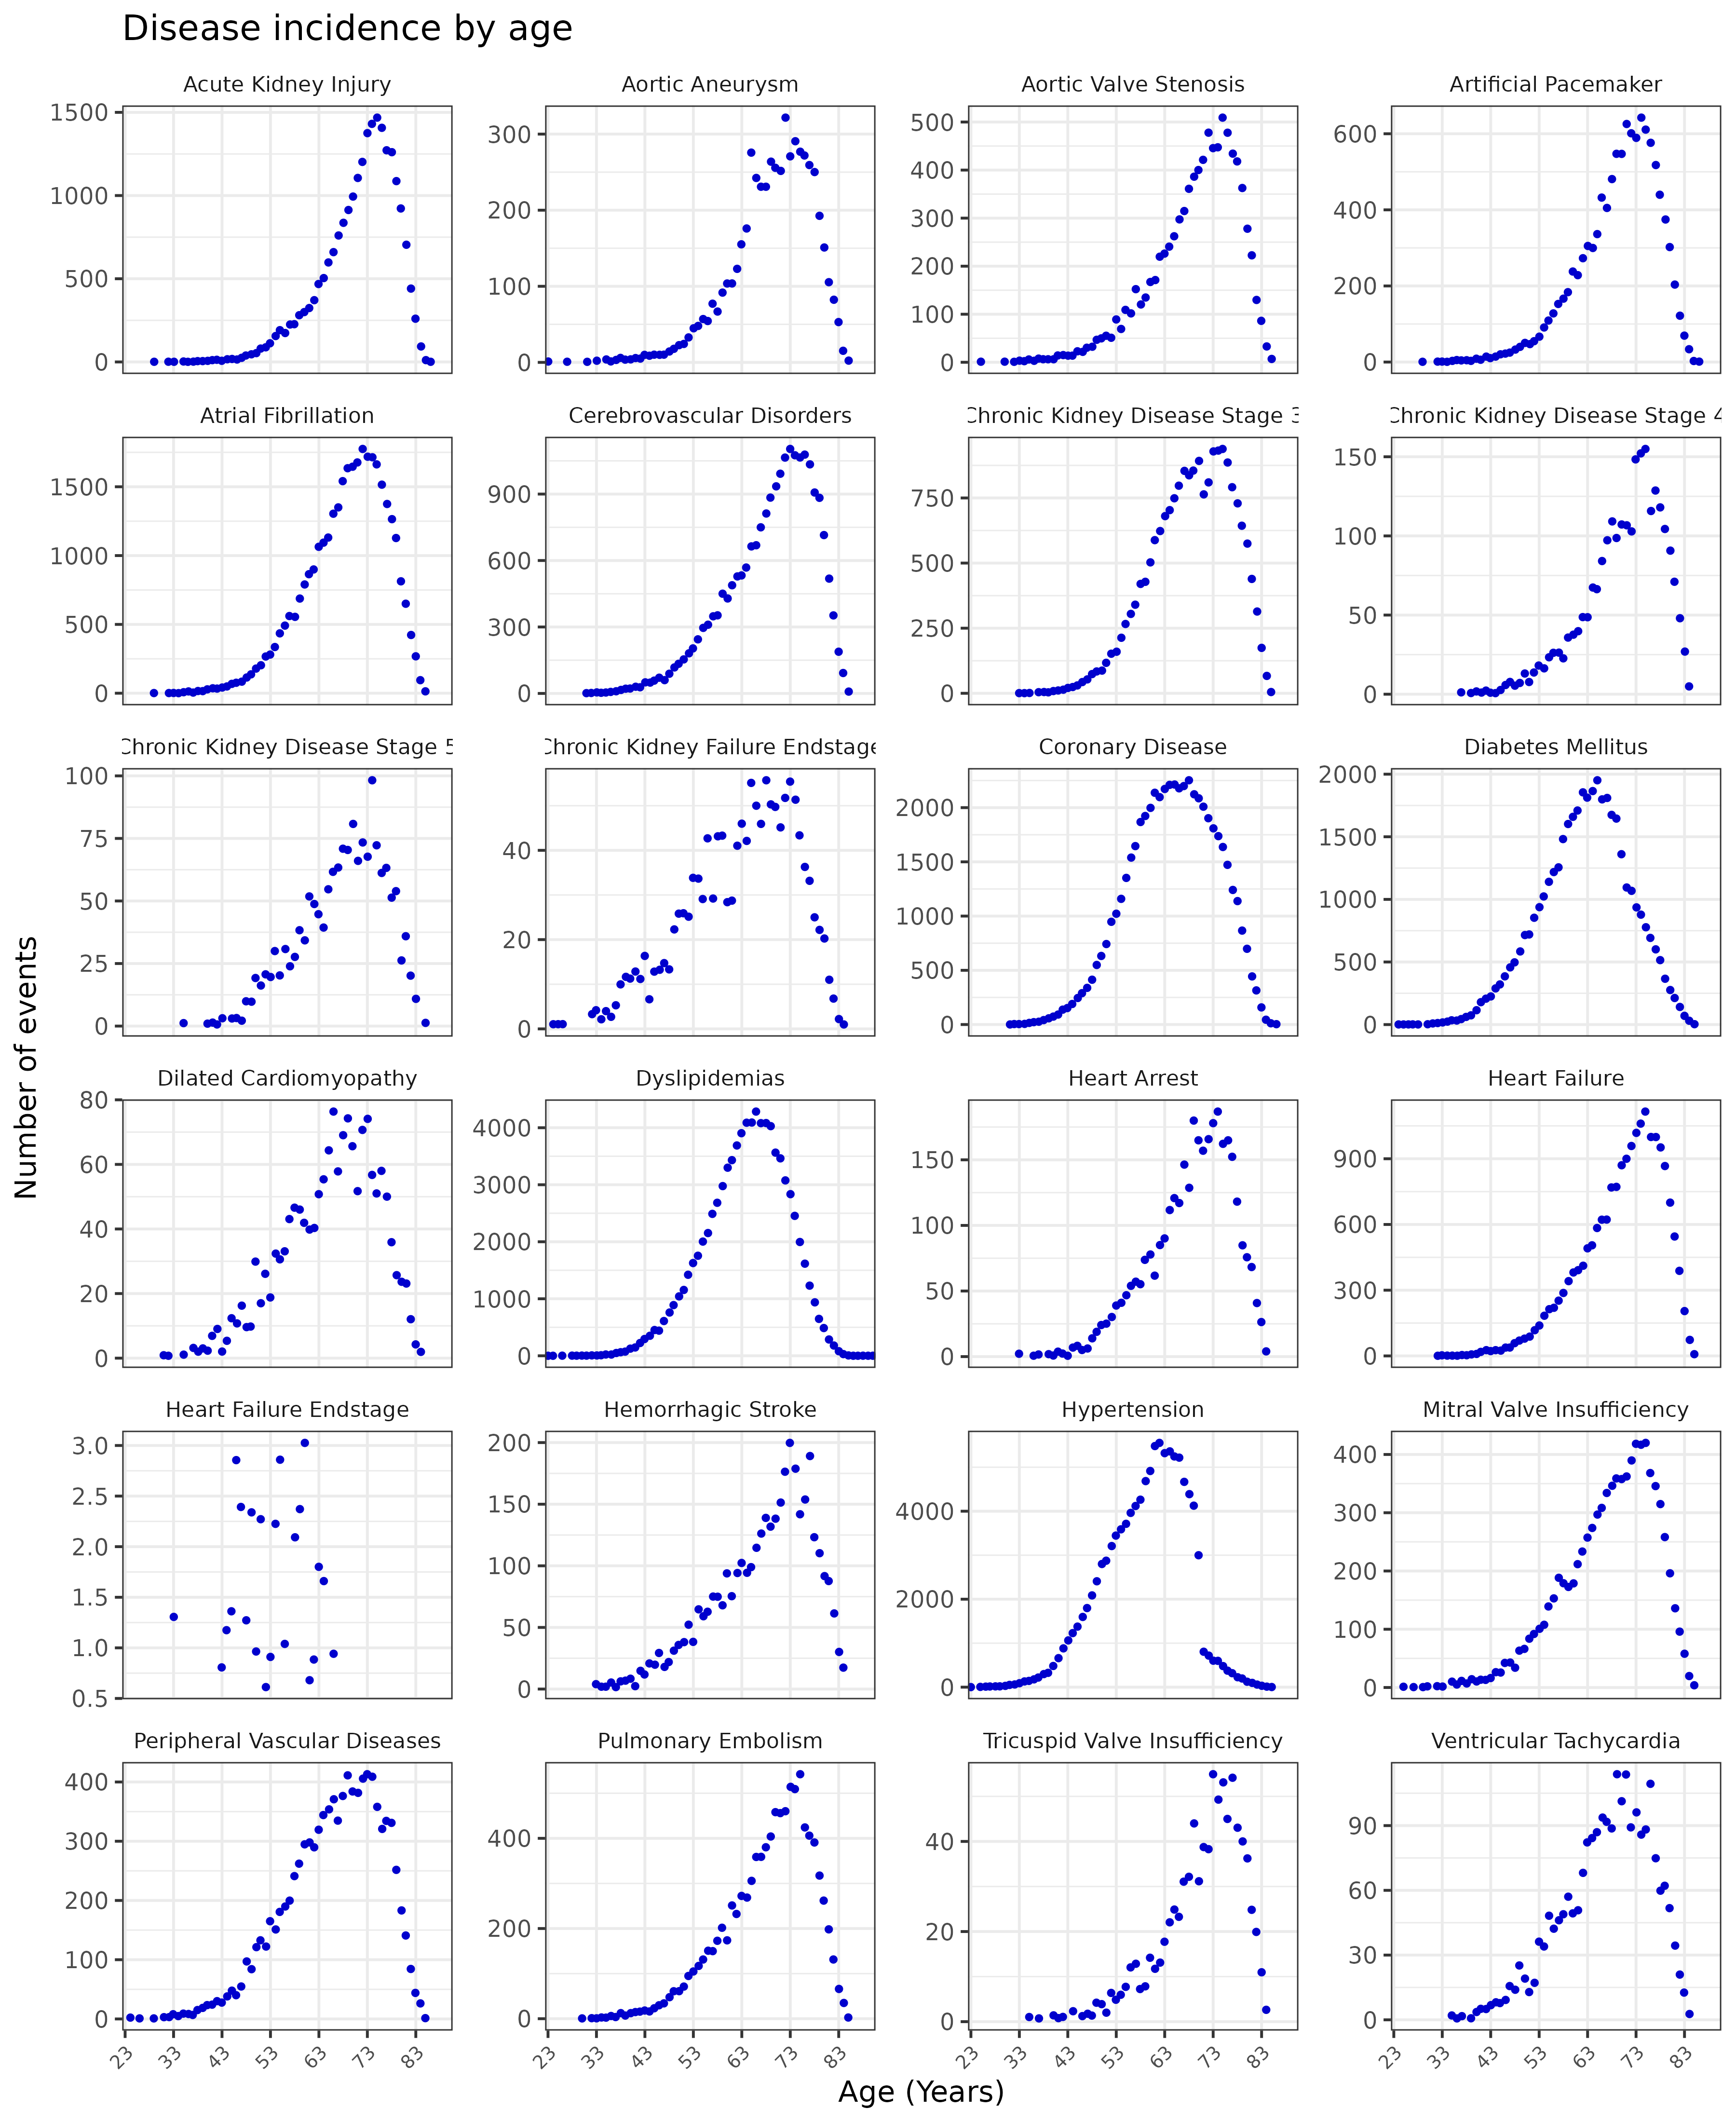
\includegraphics[width=0.8\textwidth]{Figures/disease_incidence_by_age.png}
    \caption{Age distribution of disease incidence across 24 primary diseases. Each panel shows the number of incident cases by age (in years) for a specific disease. The y-axis scale varies across panels to accommodate different incidence rates.}
    \label{supp_mat:SF0}
\end{figure}

\newpage

\begin{figure}[H]
    \centering
    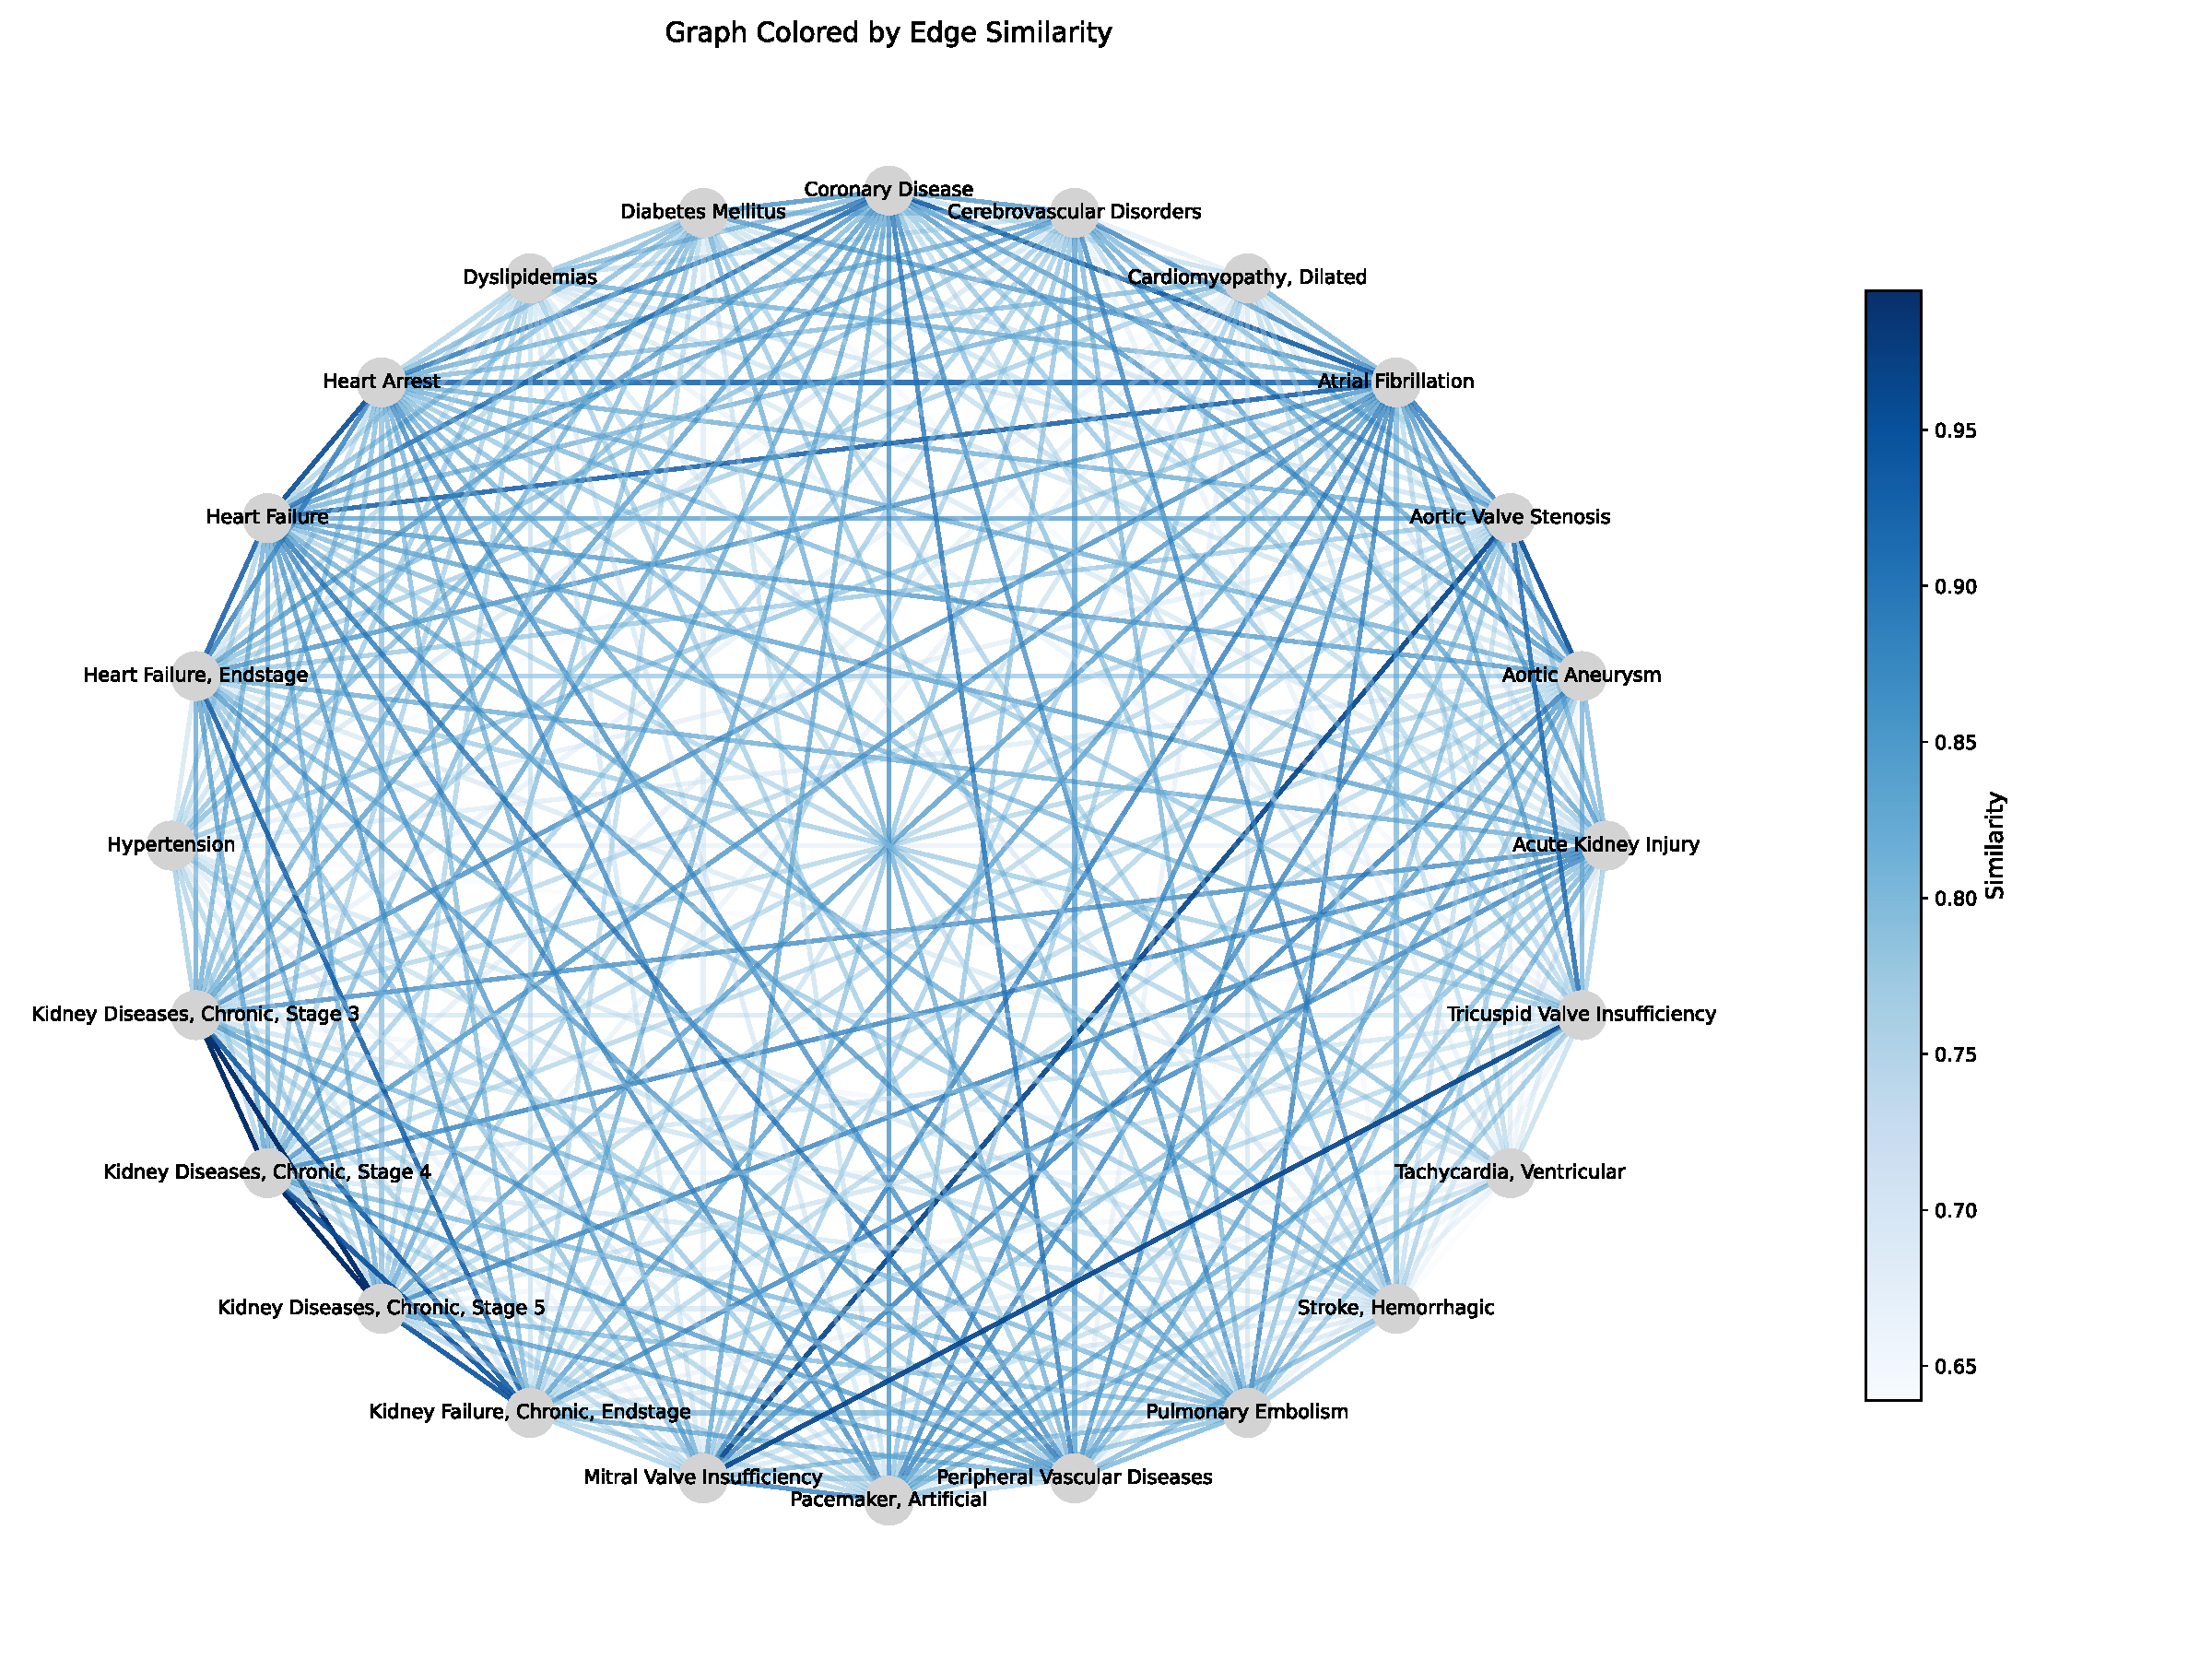
\includegraphics[width=1\textwidth]{Figures/graph_similarity_plot_main_par.pdf}
    \caption{Cosine similarity network for 24 cardiometabolic diseases computed from embeddings including both cardiometabolic diseases and risk factors. Darker colors indicate stronger similarities.}
    \label{supp_mat:SF2}
\end{figure}


\begin{figure}[H]
    \centering
    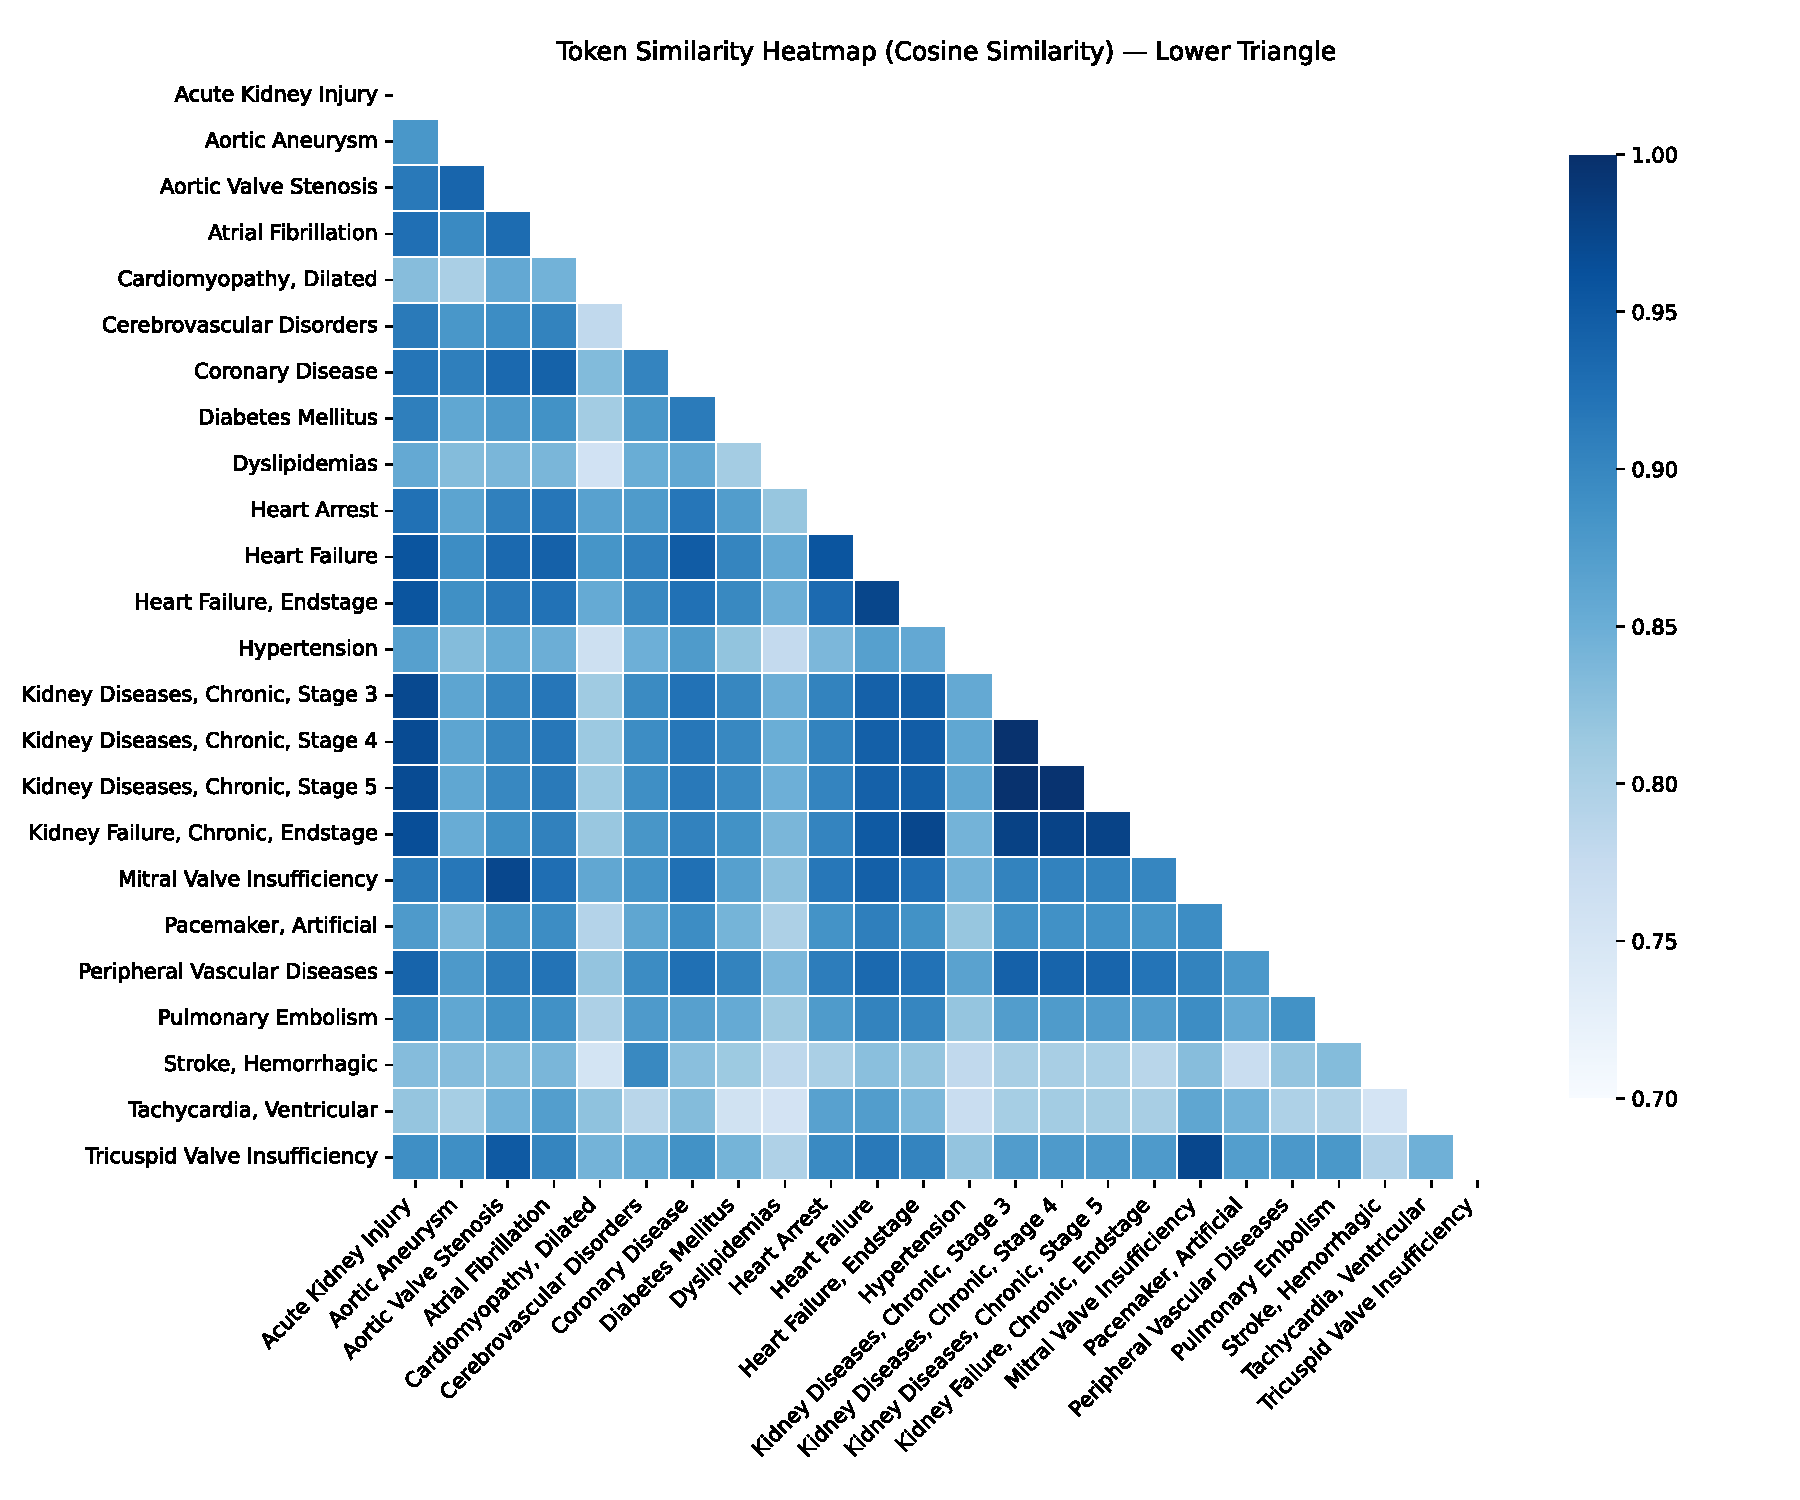
\includegraphics[width=1\textwidth]{Figures/disease_similarity_heatmap_main.pdf}
    \caption{Cosine similarity matrix for 24 cardiometabolic diseases computed from embeddings including only cardiometabolic diseases. Darker colors indicate stronger similarities.}
    \label{supp_mat:SF1}
\end{figure}



\newpage

\begin{figure}[H]
    \centering
    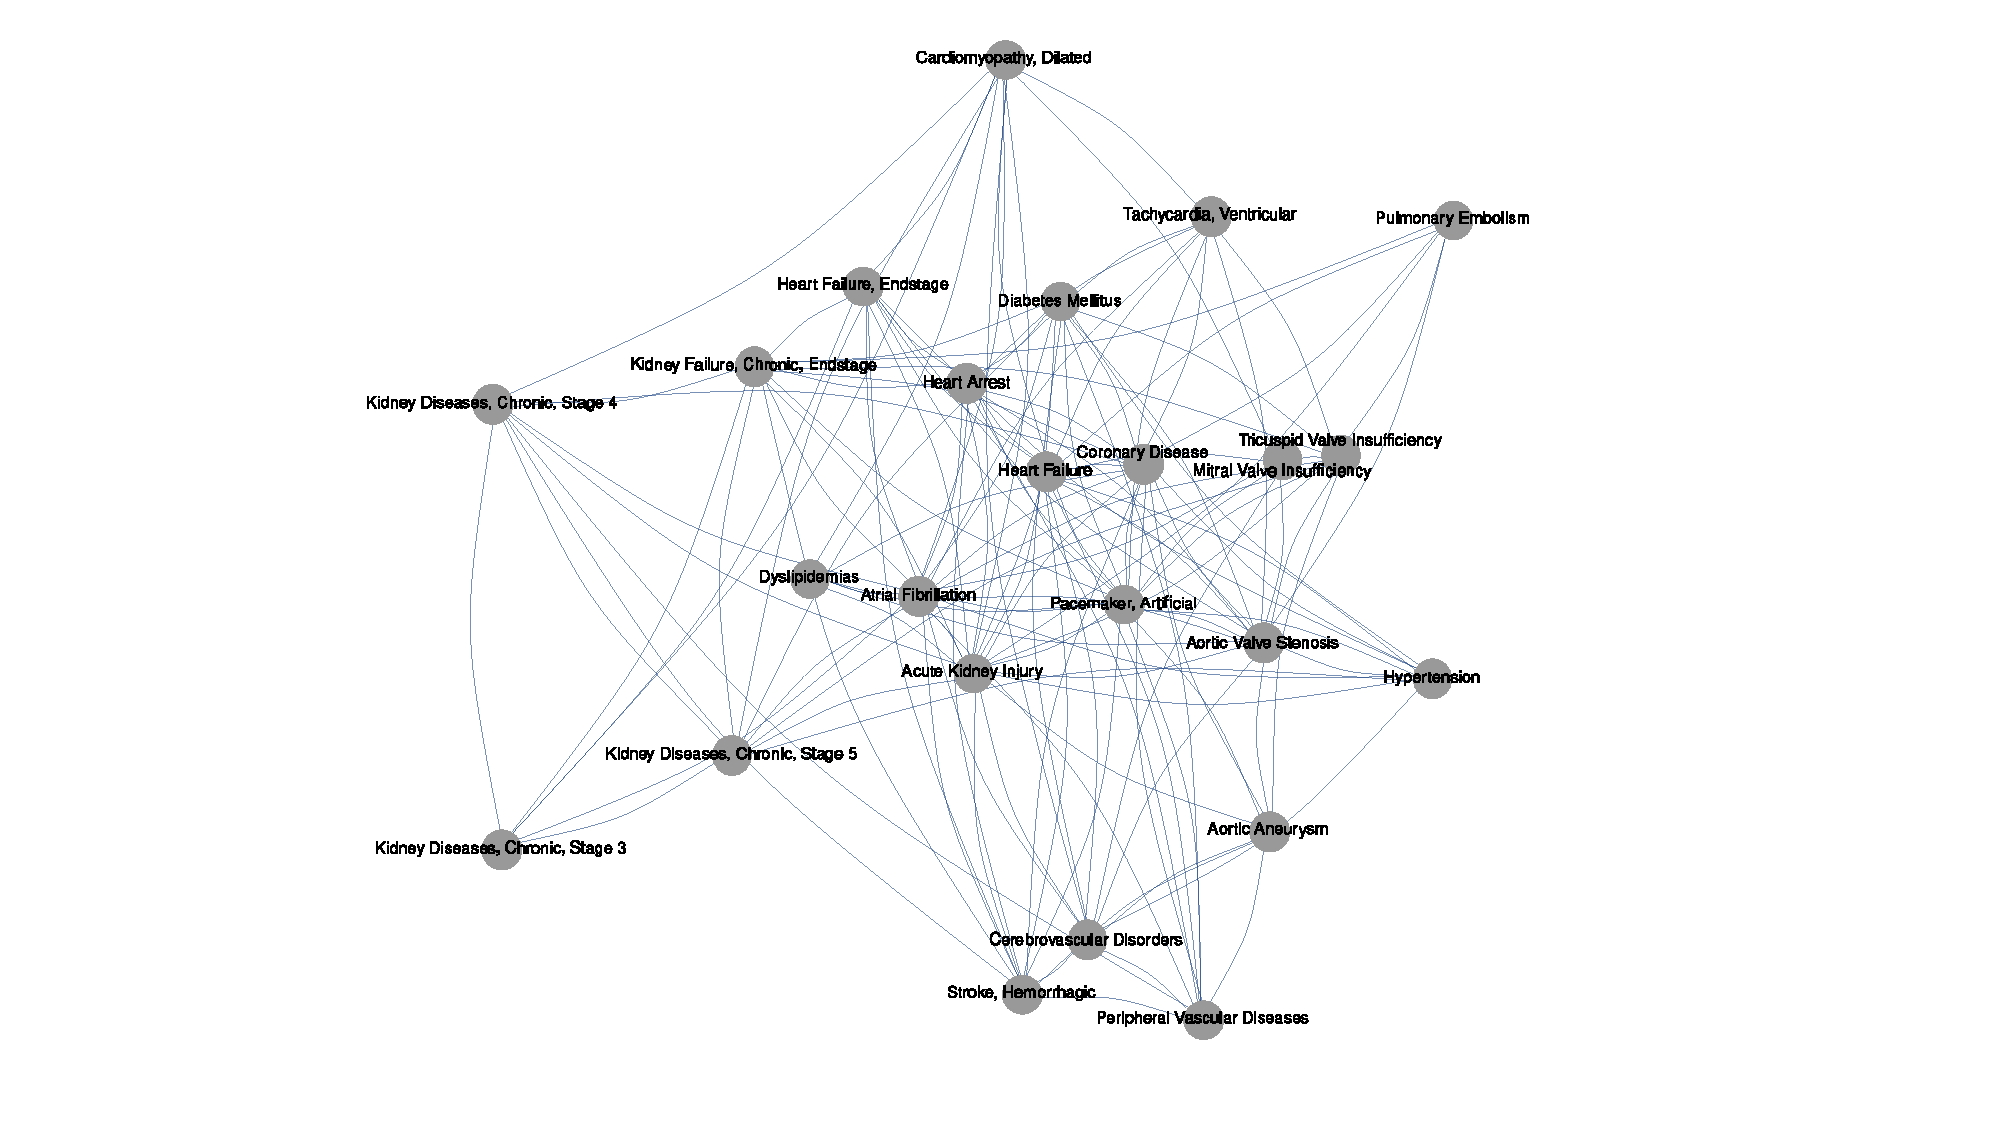
\includegraphics[width=1\textwidth]{Figures/Plots_graph_Baseline_HR.pdf}
    \caption{Cardiometabolic disease network estimated via Gaussian Graphical Lasso Regression computed from embeddings including both cardiometabolic diseases and risk factors.}
    \label{supp_mat:SF3}
\end{figure}

\clearpage